\documentclass[journal,10pt,twocolumn]{IEEEtran}

\usepackage{setspace}
\usepackage{gensymb}
\singlespacing
\usepackage[cmex10]{amsmath}

\usepackage{amsthm}

\usepackage{mathrsfs}
\usepackage{txfonts}
\usepackage{stfloats}
\usepackage{bm}
\usepackage{cite}
\usepackage{cases}
\usepackage{subfig}
\usepackage{breqn}
\usepackage{longtable}
\usepackage{multirow}
\usepackage{xfrac}
\usepackage{enumitem}
\usepackage{mathtools}
\usepackage{steinmetz}
\usepackage{tikz}
\usepackage{circuitikz}
\usepackage{verbatim}
\usepackage{tfrupee}
\usepackage[breaklinks=true]{hyperref}
\usepackage{graphicx}
\usepackage{tkz-euclide}
\usepackage{nicefrac}
\usetikzlibrary{calc,math}
\usepackage{listings}
    \usepackage{color}                                            %%
    \usepackage{array}                                            %%
    \usepackage{longtable}                                        %%
    \usepackage{calc}                                             %%
    \usepackage{multirow}                                         %%
    \usepackage{hhline}                                           %%
    \usepackage{ifthen}                                           %%
    \usepackage{lscape}     
\usepackage{multicol}
\usepackage{chngcntr}

\DeclareMathOperator*{\Res}{Res}

\renewcommand\thesection{\arabic{section}}
\renewcommand\thesubsection{\thesection.\arabic{subsection}}
\renewcommand\thesubsubsection{\thesubsection.\arabic{subsubsection}}

\renewcommand\thesectiondis{\arabic{section}}
\renewcommand\thesubsectiondis{\thesectiondis.\arabic{subsection}}
\renewcommand\thesubsubsectiondis{\thesubsectiondis.\arabic{subsubsection}}


\hyphenation{op-tical net-works semi-conduc-tor}
\def\inputGnumericTable{}                                 %%

\lstset{
%language=C,
frame=single, 
breaklines=true,
columns=fullflexible
}
\begin{document}


\newtheorem{theorem}{Theorem}[section]
\newtheorem{problem}{Problem}
\newtheorem{proposition}{Proposition}[section]
\newtheorem{lemma}{Lemma}[section]
\newtheorem{corollary}[theorem]{Corollary}
\newtheorem{example}{Example}[section]
\newtheorem{definition}[problem]{Definition}

\newcommand{\BEQA}{\begin{eqnarray}}
\newcommand{\EEQA}{\end{eqnarray}}
\newcommand{\define}{\stackrel{\triangle}{=}}
\bibliographystyle{IEEEtran}
\raggedbottom
\setlength{\parindent}{0pt}
\providecommand{\mbf}{\mathbf}
\providecommand{\pr}[1]{\ensuremath{\Pr\left(#1\right)}}
\providecommand{\qfunc}[1]{\ensuremath{Q\left(#1\right)}}
\providecommand{\sbrak}[1]{\ensuremath{{}\left[#1\right]}}
\providecommand{\lsbrak}[1]{\ensuremath{{}\left[#1\right.}}
\providecommand{\rsbrak}[1]{\ensuremath{{}\left.#1\right]}}
\providecommand{\brak}[1]{\ensuremath{\left(#1\right)}}
\providecommand{\lbrak}[1]{\ensuremath{\left(#1\right.}}
\providecommand{\rbrak}[1]{\ensuremath{\left.#1\right)}}
\providecommand{\cbrak}[1]{\ensuremath{\left\{#1\right\}}}
\providecommand{\lcbrak}[1]{\ensuremath{\left\{#1\right.}}
\providecommand{\rcbrak}[1]{\ensuremath{\left.#1\right\}}}
\theoremstyle{remark}
\newtheorem{rem}{Remark}
\newcommand{\sgn}{\mathop{\mathrm{sgn}}}
\providecommand{\abs}[1]{\left\vert#1\right\vert}
\providecommand{\res}[1]{\Res\displaylimits_{#1}} 
\providecommand{\norm}[1]{\left\lVert#1\right\rVert}
%\providecommand{\norm}[1]{\lVert#1\rVert}
\providecommand{\mtx}[1]{\mathbf{#1}}
\providecommand{\mean}[1]{E\left[ #1 \right]}
\providecommand{\fourier}{\overset{\mathcal{F}}{ \rightleftharpoons}}
%\providecommand{\hilbert}{\overset{\mathcal{H}}{ \rightleftharpoons}}
\providecommand{\system}{\overset{\mathcal{H}}{ \longleftrightarrow}}
	%\newcommand{\solution}[2]{\textbf{Solution:}{#1}}
\newcommand{\solution}{\noindent \textbf{Solution: }}
\newcommand{\cosec}{\,\text{cosec}\,}
\providecommand{\dec}[2]{\ensuremath{\overset{#1}{\underset{#2}{\gtrless}}}}
\newcommand{\myvec}[1]{\ensuremath{\begin{pmatrix}#1\end{pmatrix}}}
\newcommand{\mydet}[1]{\ensuremath{\begin{vmatrix}#1\end{vmatrix}}}
\numberwithin{equation}{subsection}
\makeatletter
\makeatother
\let\vec\mathbf
\def\putbox#1#2#3{\makebox[0in][l]{\makebox[#1][l]{}\raisebox{\baselineskip}[0in][0in]{\raisebox{#2}[0in][0in]{#3}}}}
     \def\rightbox#1{\makebox[0in][r]{#1}}
     \def\centbox#1{\makebox[0in]{#1}}
     \def\topbox#1{\raisebox{-\baselineskip}[0in][0in]{#1}}
     \def\midbox#1{\raisebox{-0.5\baselineskip}[0in][0in]{#1}}
\vspace{3cm}
\title{Assignment 3}
\author{Gautham Bellamkonda - CS20BTECH11017}
\maketitle
\newpage
\bigskip
\renewcommand{\thetable}{\theenumi}
Download all python codes from 
\begin{lstlisting}
https://github.com/GauthamBellamkonda/AI1103/tree/main/Assignment3/Codes
\end{lstlisting}
and latex-tikz codes from 
\begin{lstlisting}
https://github.com/GauthamBellamkonda/AI1103/tree/main/Assignment3
\end{lstlisting}
\section{Problem}
(GATE 45) Consider a discrete-time channel $Y = X + Z$, where the additive noise $Z$ is signal dependent. In particular, given the transmitted symbol $X \in \{-a, a \}$ at any instant, the noise sample $Z$ is chosen indepedently from a Gaussian distribution with mean $\beta X$ and unit variance. Assume a threshold detector with zero threshold at the receiver. When $\beta = 0$, the BER was found to be $Q(a) = 1 \times 10^{-8}.$
\begin{align}
\left( Q(v) = \dfrac{1}{\sqrt{2 \pi}} \int_v ^{\infty} e^{-\frac{u^2}{2}} du \text{, and for } v > 1 \text{, use } Q(v) = e^{\frac{-v^2}{2}} \right)
\end{align}
When $\beta = -0.3$, BER is closest to
\begin{enumerate}[label = (\Alph*)]
\item $10^{-7}$
\item $10^{-6}$
\item $10^{-4}$ \label{option C}
\item $10^{-2}$
\end{enumerate}
\section{Solution}
Given that the threshold of the detector is zero. Define a detector function $g$ such that
\begin{align}
g(Y) = 
\begin{cases}
+a & Y>0 \\
-a & Y<0
\end{cases}
\end{align}
It is given that $X \in \{ -a, a\}$ is a random variable.
\begin{align}
\therefore \Pr(X=a) = \Pr(X=-a) = \dfrac{1}{2}
\end{align}
Since the noise in the signal, $Z$ is chosen independently from a Gaussian distribution with mean $ \mu = \beta X$ and unit variance, it follows that
\begin{align}
F_Z(z) &= \int_{-\infty}^{z} \dfrac{1}{\sqrt{2\pi}} \exp \left( \dfrac{-(z - \beta X)^2}{2} \right) dz \\
&= \int_{-\infty}^{z - \beta X} \dfrac{1}{\sqrt{2\pi}} \exp \left( \dfrac{-z^2}{2} \right) dz \\
&= \int_{\beta X-z}^{\infty} \dfrac{1}{\sqrt{2\pi}} \exp \left( \dfrac{-z^2}{2} \right) dz \\
&= Q(\beta X - z) \label{eqn 2.0.7}
\end{align}
Also, it is easy to see that 
\begin{align}
Q(-v) = 1 - Q(v) \; \forall \; v \in \mathbb{R} \label{eqn 2.0.8}
\end{align}
The detector can record erroneous bits in the signal iff
\begin{align}
X>0 \; &, \; g(Y) = -a \; (\text{Call this BER}_{+a}) \text{ or}\\
X<0 \; &, \; g(Y) = a \; (\text{Call this BER}_{-a})
\end{align}
\begin{align}
\therefore \text{BER}_{+a} % &= \Pr(g(Y) = -a \;,\; X = a)\\
&= \Pr(g(Y) = -a \;|\; X = a) \Pr(X=a)\\
&= \Pr(Y < 0 \;|\; X = a) \Pr(X=a)\\
&= \dfrac{1}{2} \times \Pr(X+Z < 0 \;|\; X = a) \\
% &= \dfrac{1}{2} \times \Pr(a+Z < 0 \;|\; X = a) \\
% &= \dfrac{1}{2} \times \Pr(Z < -a \;|\; X = a) \\
&= \dfrac{1}{2} \times F_Z(-a)\\
&= \dfrac{1}{2} \times Q(\beta X + a) \; \text{ (From (\ref{eqn 2.0.7}))}\\
% &= \dfrac{1}{2} \times Q(a \beta + a)\\
&= \dfrac{1}{2} \times Q(a(1+\beta))
\end{align}
\begin{align}
\text{BER}_{-a} % &= \Pr(g(Y) = a \;,\; X = -a)\\
&= \Pr(g(Y) = a \;|\; X = -a) \Pr(X=-a)\\
&= \Pr(Y > 0 \;|\; X = -a) \Pr(X=-a)\\
&= \dfrac{1}{2} \times \Pr(X+Z > 0 \;|\; X = -a) \\
% &= \dfrac{1}{2} \times \Pr(Z-a > 0 \;|\; X = -a) \\
% &= \dfrac{1}{2} \times \Pr(Z > a \;|\; X = -a) \\
&= \dfrac{1}{2} \times \left( 1 - F_Z(a) \right) \\
&= \dfrac{1}{2} \times \left( 1 - Q(\beta X -a) \right) \; \text{ (From (\ref{eqn 2.0.7}))}\\
% &= \dfrac{1}{2} \times \left( 1 - Q(-a \beta -a) \right) \\
&= \dfrac{1}{2} \times Q(a(1+\beta)) \; \text{ (From (\ref{eqn 2.0.8}))}
\end{align}
\begin{align}
\therefore \text{BER} &= \text{BER}_{+a} + \text{BER}_{-a}\\
&= Q(a(1+\beta))
\end{align} 
\begin{figure}[!hbt]
    \centering
	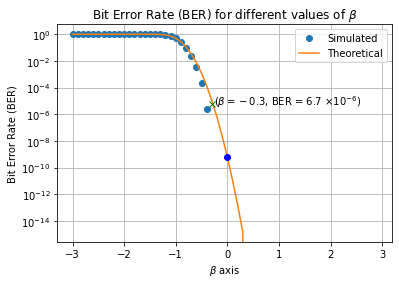
\includegraphics[width=\columnwidth]{./Figures/Figure_3.png}
    \caption{Theory vs Simulated plot of BER}
    \label{CDF_Y}
\end{figure}
When $\beta = 0$, it is given that 
\begin{align}
\text{BER} = Q(a) &= 10^{-8}
\end{align}
On computing, $Q(1) \approx 0.16$. Since $Q(a)<Q(1)$, it is easy to see that $a>1$ (as $Q(x)$ is a decreasing function)
\begin{align}
\therefore e^{-a^2 / 2} &= 10^{-8}\\
\Leftrightarrow a &\approx 6.069
\end{align}
When $\beta = -0.3$,
\begin{align}
\text{BER} = Q(a(1+\beta)) &= Q(6.069 \times (1-0.3))\\
&= Q(6.069 \times 0.7)\\
&= Q(4.249)\\
&\approx \exp (-\dfrac{4.249^2}{2})\\
&\approx 1.2 \times 10^{-4}
\end{align}
Therefore, when $\beta = -0.3$, BER is closest to $10^{-4}$ and option \ref{option C} is correct.
\end{document}
